\label{sec:experiments}

\subsection{Toy Problem -- Annulus}
\label{sec:annulus}
We first demonstrate our approach on a toy problem.
The true generative model of the observed data is a constant speed circular orbit around the origin in the $x$-$y$ plane, such that $\mathbf{x}_t = \left\lbrace x_t, y_t, \dot{x}_t, \dot{y}_t \right\rbrace \in  \mathbb{R}^4$.
To analyze this data we use a misspecified model that only simulates linear forward motion.
To overcome the model mismatch and fit the observed data, we add Gaussian noise to position and velocity.
We impose a failure constraint limiting the change in the distance of the point from the origin to a fixed threshold.
This condition mirrors our observation that states in brittle simulators have large allowable perturbations in particular directions, but very narrow permissible perturbations in other directions.
The true radius is unknown and so we must amortize over possible radii.


\begin{figure}[h!]
\centering

    \begin{subfigure}[t]{0.48\textwidth}
    \centering
        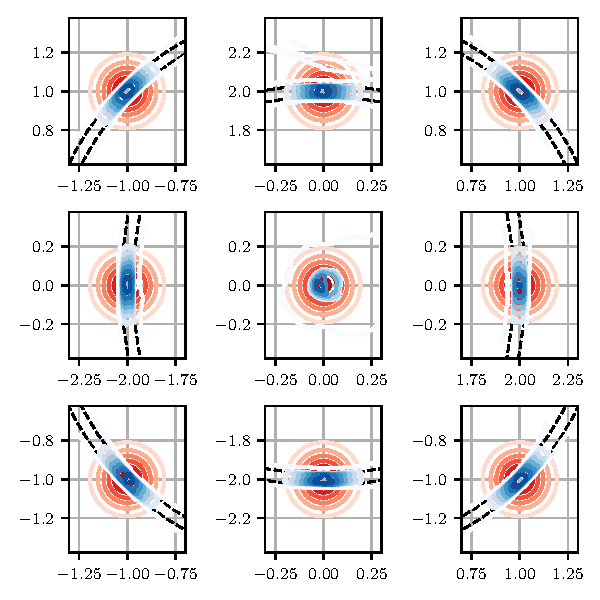
\includegraphics[width=0.95\textwidth]{figures/RNF_cluster_2019_09_26_12_27_27/RNF_density_array_1balls_00_00000_line.pdf}
        \vspace*{-0.2cm}
        \caption{}
        \label{fig:ring:space}
    \end{subfigure}%

    \begin{subfigure}[t]{0.24\textwidth}
        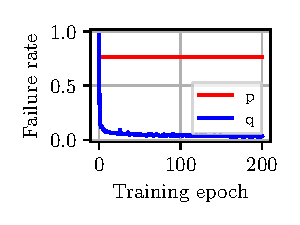
\includegraphics[width=\textwidth]{figures/RNF_cluster_2019_09_26_12_27_27/nf_bot_rate.pdf}
        \vspace*{-0.7cm}
        \caption{}
        \label{fig:ring:ar}
    \end{subfigure}%
    ~%
    \begin{subfigure}[t]{0.24\textwidth}
        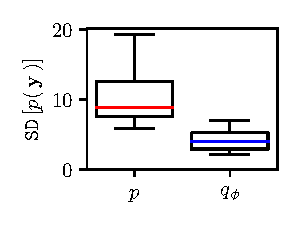
\includegraphics[width=\textwidth]{figures/RNF_cluster_2019_09_26_12_27_27/smc_variance_plot.pdf}
        \vspace*{-0.7cm}
        \caption{}
        \label{fig:ring:smc:var}
    \end{subfigure}
\vspace*{-0.2cm}
\caption{Results for the annulus problem introduced in Section \ref{sec:annulus}, where the acceptable region of perturbations is inside the black dashed band.
\ref{fig:ring:space} shows in blue the learned state-dependent proposal distribution over velocity (for a state at rest) is the well-approximating the original proposal (shown in red) \emph{inside} the acceptable region, with minimal mall in the invalid region, all but eliminating rejection as shown in \ref{fig:ring:ar}.
\ref{fig:ring:smc:var} shows the reduction in the variance of the evidence by using $q_{\phi}$.
We compute the variance using $100$ independent SMC sweeps, each using $100$ particles, and compare across $100$ datasets.
}
\label{fig:ring}
\end{figure}


The results of this experiment are shown in Figure~\ref{fig:ring}.
The interior of the black dashed lines in Figure~\ref{fig:ring:space} indicates the permissible $\dot{x}$-$\dot{y}$ perturbation, for the given position and zero velocity, where we have centered each distribution on the current position for ease of visual inspection.
Red contours indicate the original density $p(\mathbf{z}_t | \mathbf{x}_{t-1})$, and blue contours indicate the learned density $q_{\phi}(\mathbf{z}_t | \mathbf{x}_{t-1})$.
The fraction of the probability mass outside the black dashed region is the expected rejection rate.
Figure~\ref{fig:ring:ar} shows the rejection rate drops from approximately $75\%$ under the original model to approximately $4\%$ using a trained $q_{\phi}$.

\begin{figure}[h!]
    \centering
    
    \begin{subfigure}[t]{0.48\textwidth}
        \begin{subfigure}[t]{\textwidth}
            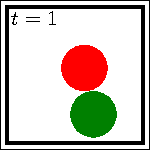
\includegraphics[width=0.22\textwidth]{figures/BBNF/BBNF3_cluster_2019_10_03_11_38_39/frame_00001.pdf}%
            ~
            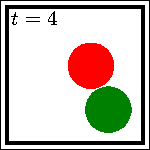
\includegraphics[width=0.22\textwidth]{figures/BBNF/BBNF3_cluster_2019_10_03_11_38_39/frame_00004.pdf}%
            ~
            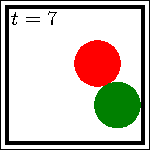
\includegraphics[width=0.22\textwidth]{figures/BBNF/BBNF3_cluster_2019_10_03_11_38_39/frame_00007.pdf}%
            ~
            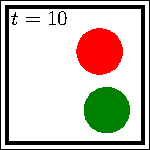
\includegraphics[width=0.22\textwidth]{figures/BBNF/BBNF3_cluster_2019_10_03_11_38_39/frame_00010.pdf}%
            % \vspace*{-0.2cm}
        \end{subfigure}
        \vspace*{-0.5cm}
        \caption{}
        \label{fig:balls:trajectory}
    \end{subfigure}%
    
    % \vspace*{-0.1cm}
    \begin{subfigure}[t]{0.48\textwidth}
        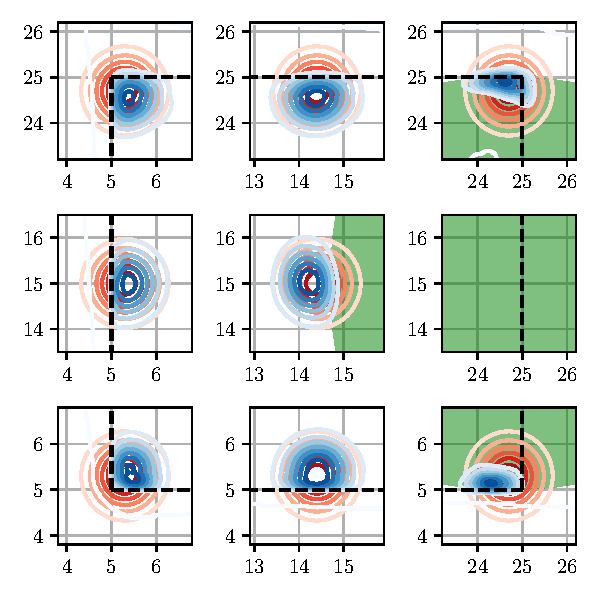
\includegraphics[width=\textwidth]{figures/BBNF/BBNF3_cluster_2019_10_03_11_38_39/BBNF3_density_array_2balls_00_000000.pdf}
        \vspace*{-0.7cm}
        \caption{}
        \label{fig:balls:space}
    \end{subfigure}%
    
    \vspace*{0.1cm}
    \begin{subfigure}[t]{0.45\textwidth}
        \begin{overpic}[width=\textwidth]{figures/BBNF/BBNF3_cluster_2019_10_03_11_38_39/bot_rate.pdf}
        \put (4, 4) {$p$}
        \put (44, 4) {$q_{\phi}$}
        \end{overpic}
        \vspace*{-0.5cm}
        \caption{}
        \label{fig:balls:rr}
    \end{subfigure}%
    \vspace*{-0.2cm}
    \caption{Results of the bouncing balls experiment introduced in Section \ref{sec:experiments:bb}, with two radius five, unit mass balls in an enclosure of size $30$.
    \ref{fig:balls:trajectory} shows an example trajectory of the system.
    \ref{fig:balls:space} shows, in red, the proposal distribution over the perturbation to the position of the first ball specified in the model, and the learned proposal in blue. The edge of the permissible region of the enclosure is shown as a black dashed line. The second ball is fixed at $\left[ 25, 15\right]$, and the induced invalid region shaded green. The flow has learned to deflect away from the disallowed regions.
    \ref{fig:balls:rr} shows the rejection rate as a function of the position of the first ball, with the second ball in the position shown. The trained proposal (right) has all but eliminated rejection in the permissible space compared to the a-priori specified proposal (left).
    The rejection rate under $p$ is high in the interior as the second ball may also leave the enclosure, whereas $q_{\phi}$ has practically eliminated rejection by \emph{jointly} proposing perturbations.}
    \label{fig:balls}
\end{figure}

We then use the learned $q_{\phi}$ as the perturbation proposal in an SMC sweep, where we condition on noisy observations of the $x$-$y$ coordinates.
As we focus on the sample efficiency of the sweep, we fix the number of calls to the simulator in Algorithm \ref{alg:rs} to a single call, instead of proposing and rejecting until acceptance.
Failed particles are then not resampled (with certainty) during the resampling.
This means that each iteration of the SMC makes a fixed number of calls to the simulator, and hence we can compare algorithms under a fixed sample budget.
Figure \ref{fig:ring:smc:var} shows that we recover lower variance evidence approximations for a fixed sample budget by using $q_{\phi}$ instead of $p$.
A paired t-test evaluating the difference in variance returns a p-value of less than $0.0001$, indicating a strong statistical difference between the performance under $p$ and $q_{\phi}$, confirming that using $q_{\phi}$ increases the fidelity of inference for a fixed sample budget.

\subsection{Bouncing Balls}
\label{sec:experiments:bb}
Our second example uses a simulator of balls bouncing elastically, as shown in Figure \ref{fig:balls:trajectory}.
We model the position and velocity of each ball, such that the dimensionality of the state vector, $\mathbf{x}_t$, is four times the number of balls.
We add a small amount of Gaussian noise at each iteration to the position and velocity of each ball.
This perturbation induces the possibility that two balls overlap, or, a ball intersects with the wall, representing an invalid physical configuration and results in simulator failure.
We note that here, we are conditioning on the state of \emph{all} balls simultaneously, and proposing the perturbation to the state \emph{jointly}.

Figure \ref{fig:balls:space} shows the distribution over position perturbation of a single ball, conditioned on the other ball being stationary.
Blue contours show the estimated distribution over accepted perturbations learned by autoregressive flow.
Figure \ref{fig:balls:rr} shows the rejection rate under $p$ and $q_{\phi}$ as a function of the position of the first ball, with the second ball fixed in the position shown, showing that rejection has been all but eliminated.
We again see a reduction in the variance of the evidence approximation computed by a particle filter when using $q_{\phi}$ instead of $p$ (figure in the supplementary materials).

\subsection{MuJoCo}
\label{sec:experiments:tosser}
We now apply our method to the popular robotics simulator MuJoCo~\citep{todorov2012mujoco}, specifically using the built-in example ``tosser,'' where a capsule is ``tossed'' by an actuator into a bucket, shown in Figure \ref{fig:tosser:im}.
Tosser displays ``choatic'' aspects, as minor changes in the position of the object results in large changes in the trajectories achieved by the simulator.

MuJoCo allows some overlap between the objects to simulate contact dynamics. 
This is an example of model misspecification borne out of the requirements of reasonably writing a simulator.
We therefore place a hard limit on the amount objects are allowed to overlap.
This is an example of a user-specified constraint that requires the simulator to be run to evaluate.
We add Gaussian distributed noise to the position and velocity of the capsule.

\begin{figure}[t]
    \centering
    
    \begin{subfigure}[t]{0.48\textwidth}
        \centering
        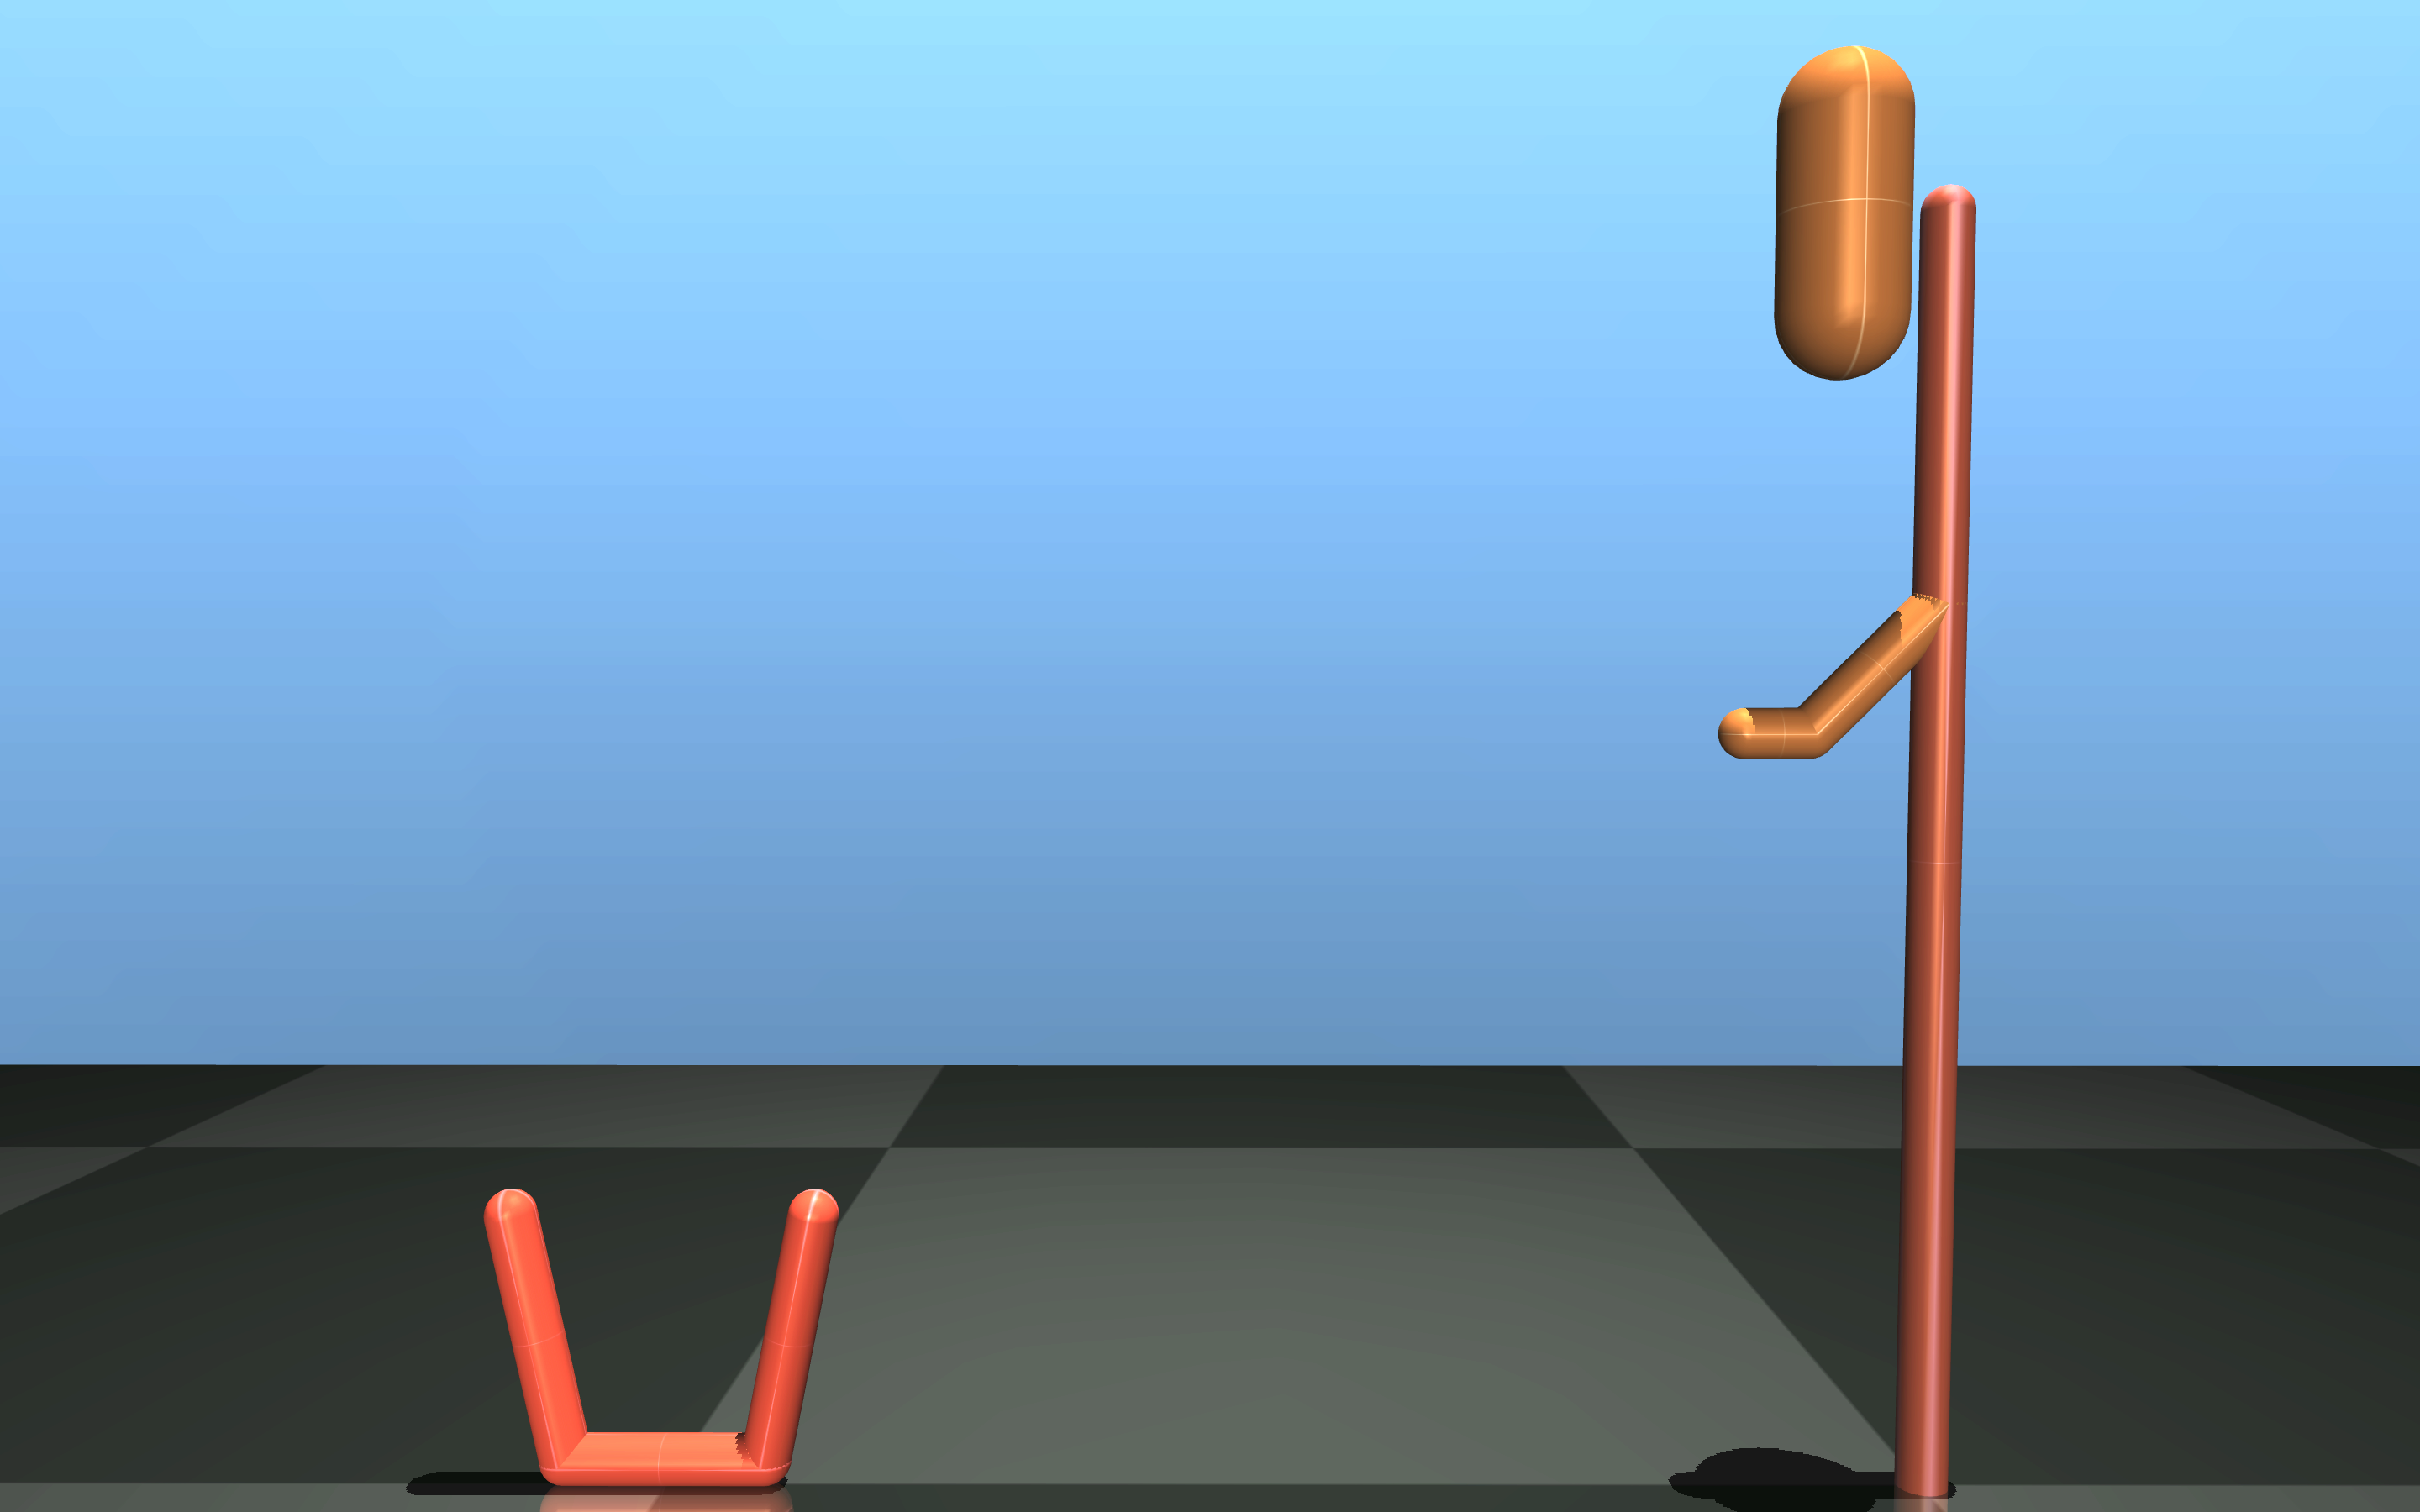
\includegraphics[width=0.24\textwidth]{figures/tosser/tosser1.png}%
        ~%
        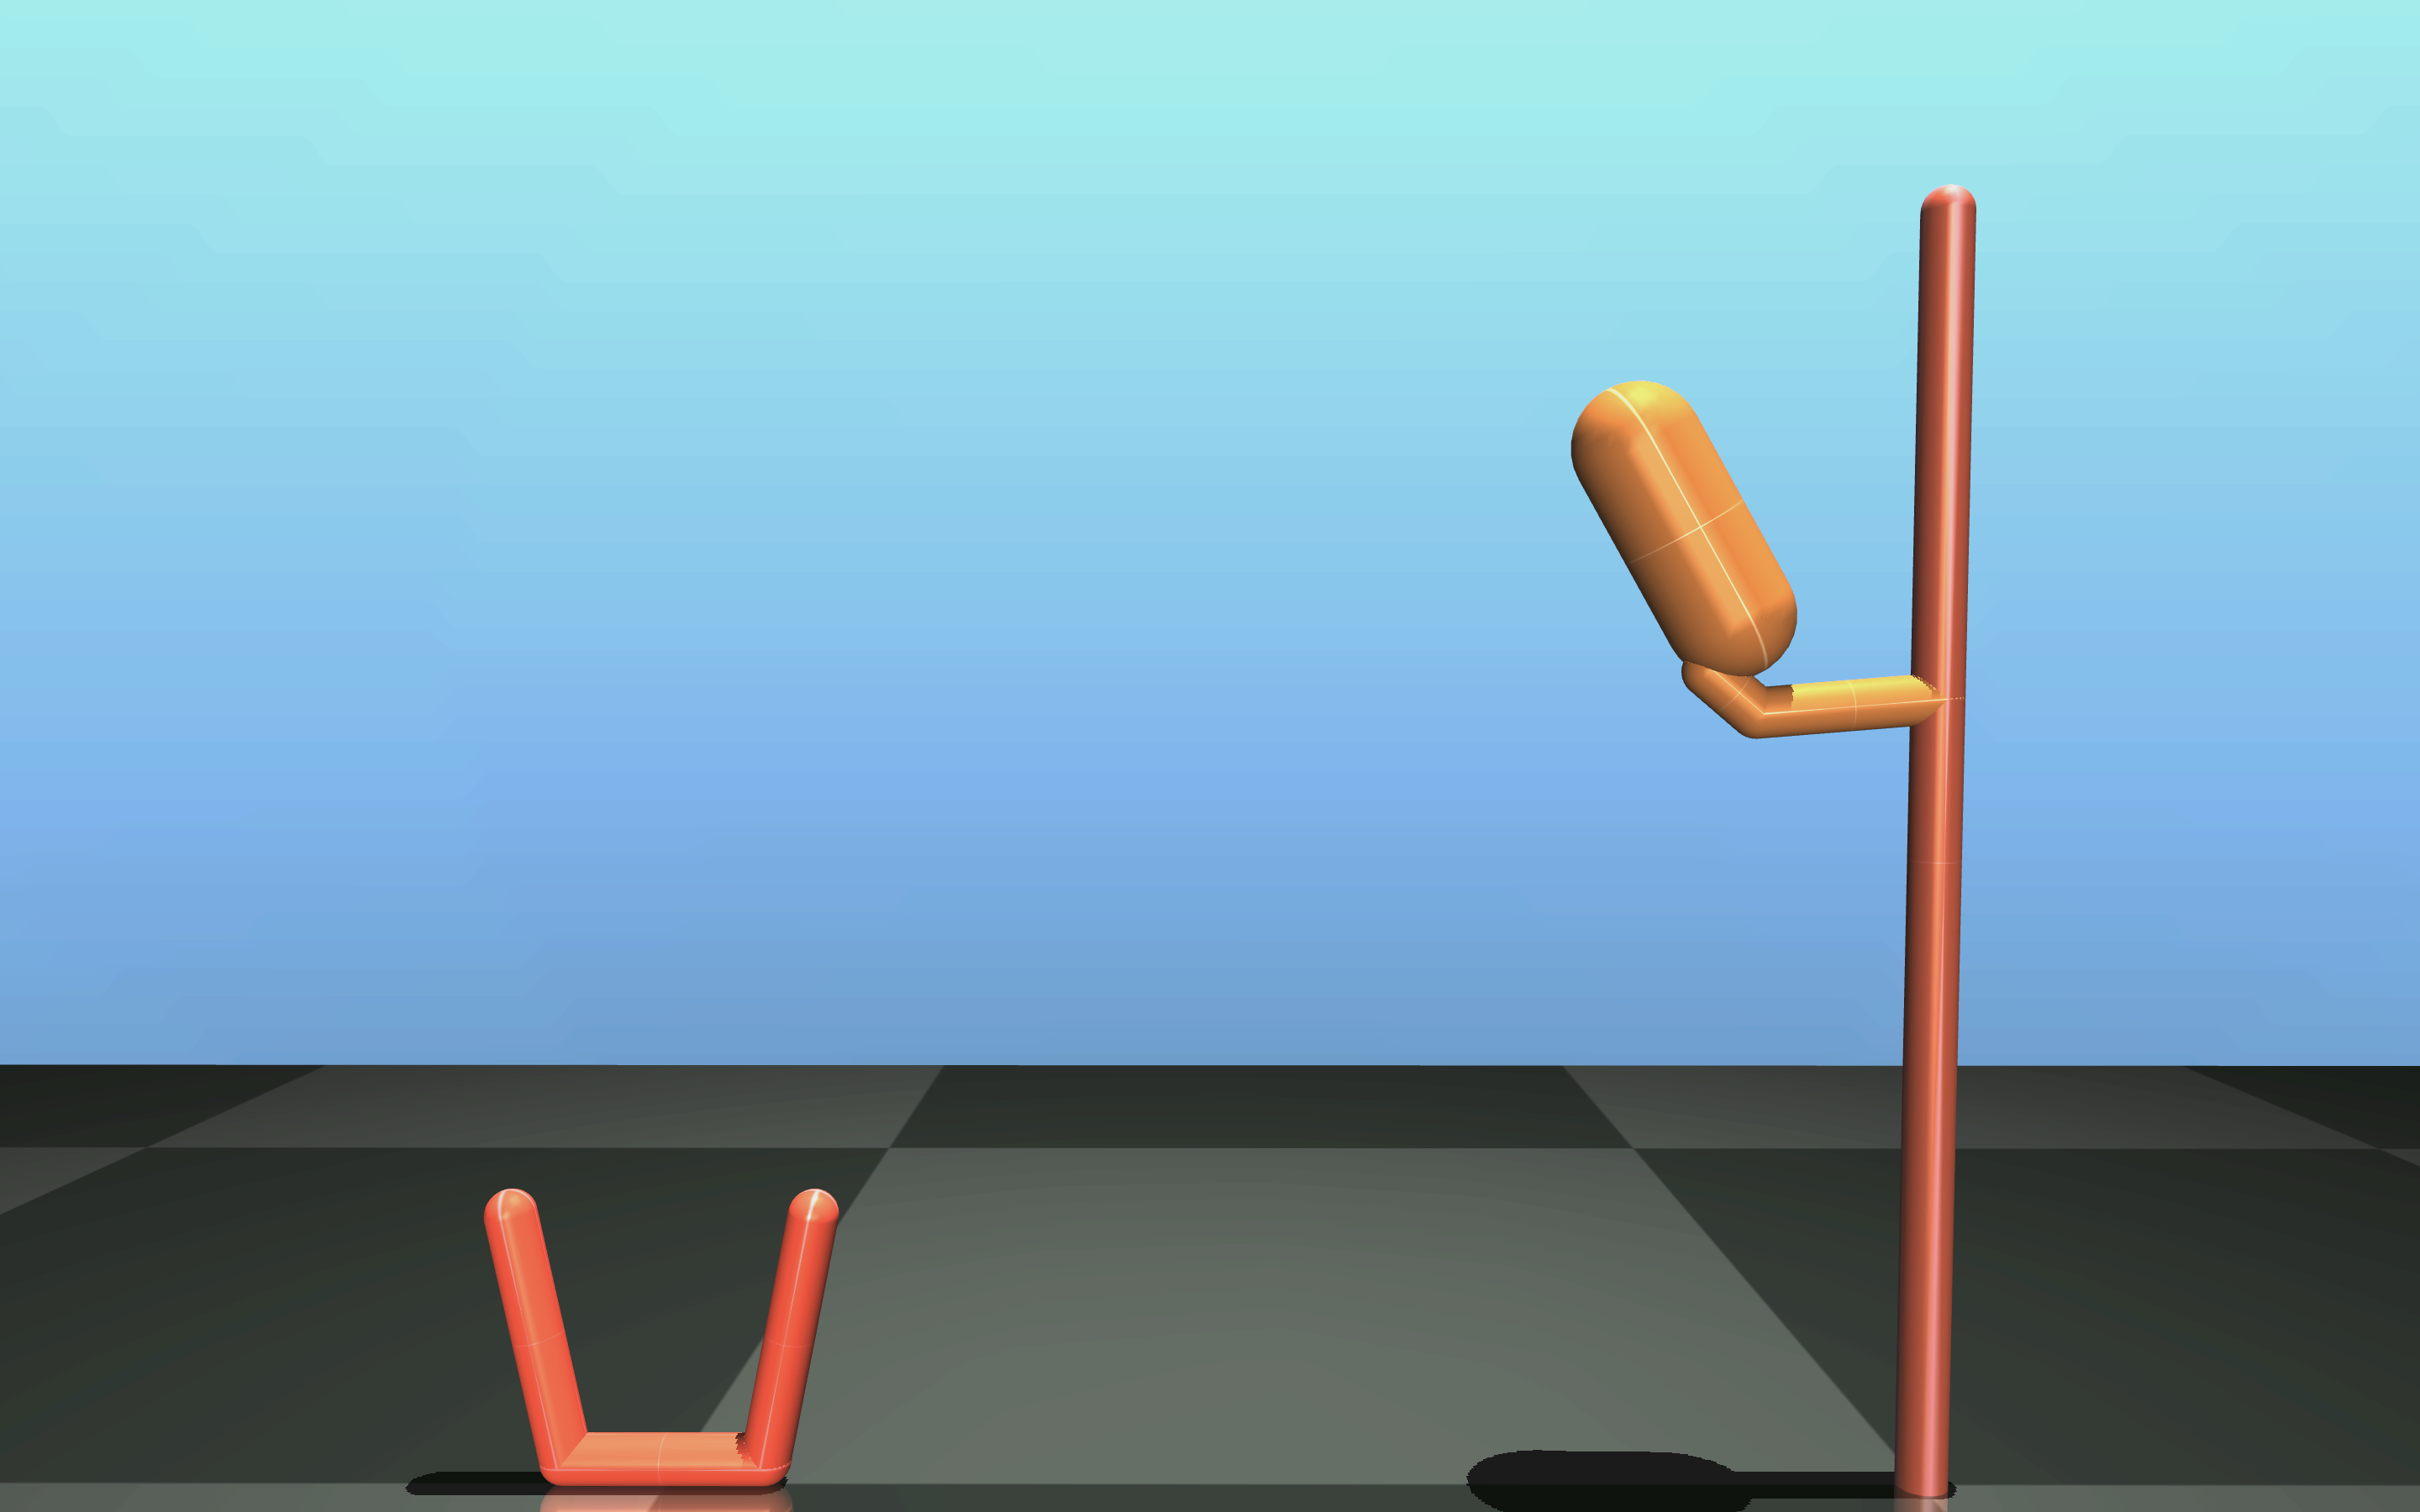
\includegraphics[width=0.24\textwidth]{figures/tosser/tosser2.png}%
        ~%
        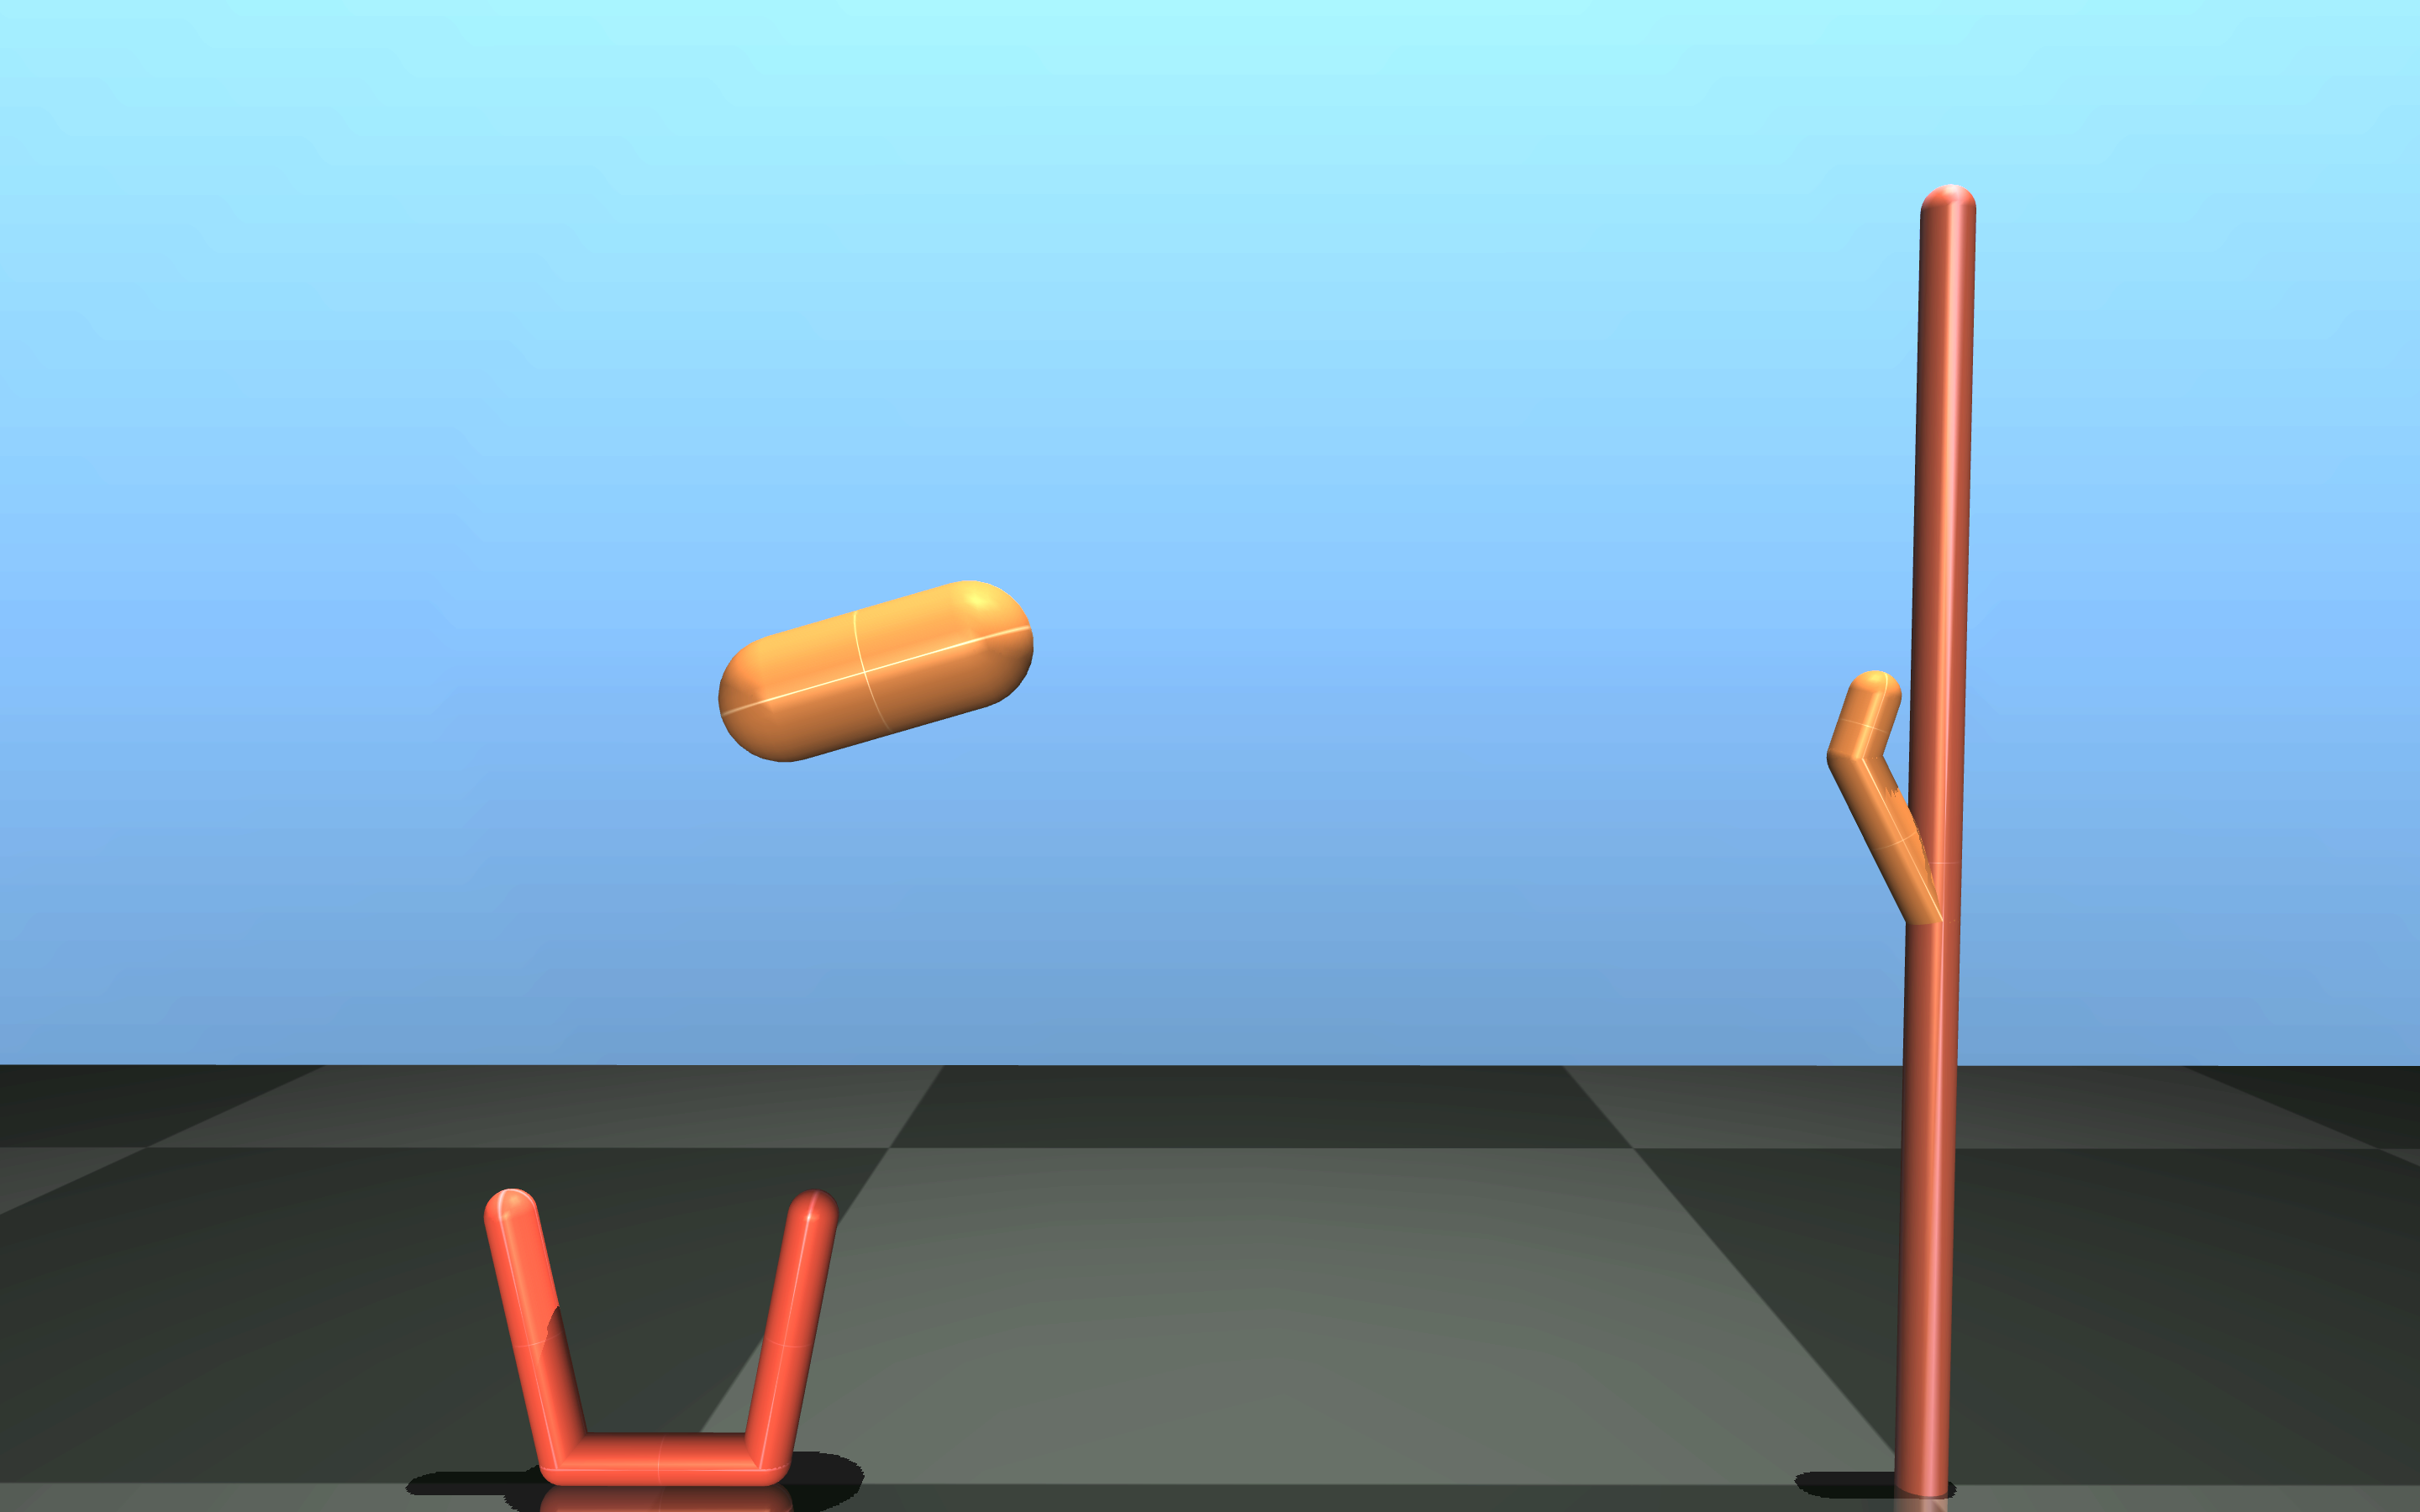
\includegraphics[width=0.24\textwidth]{figures/tosser/tosser3.png}%
        ~%
        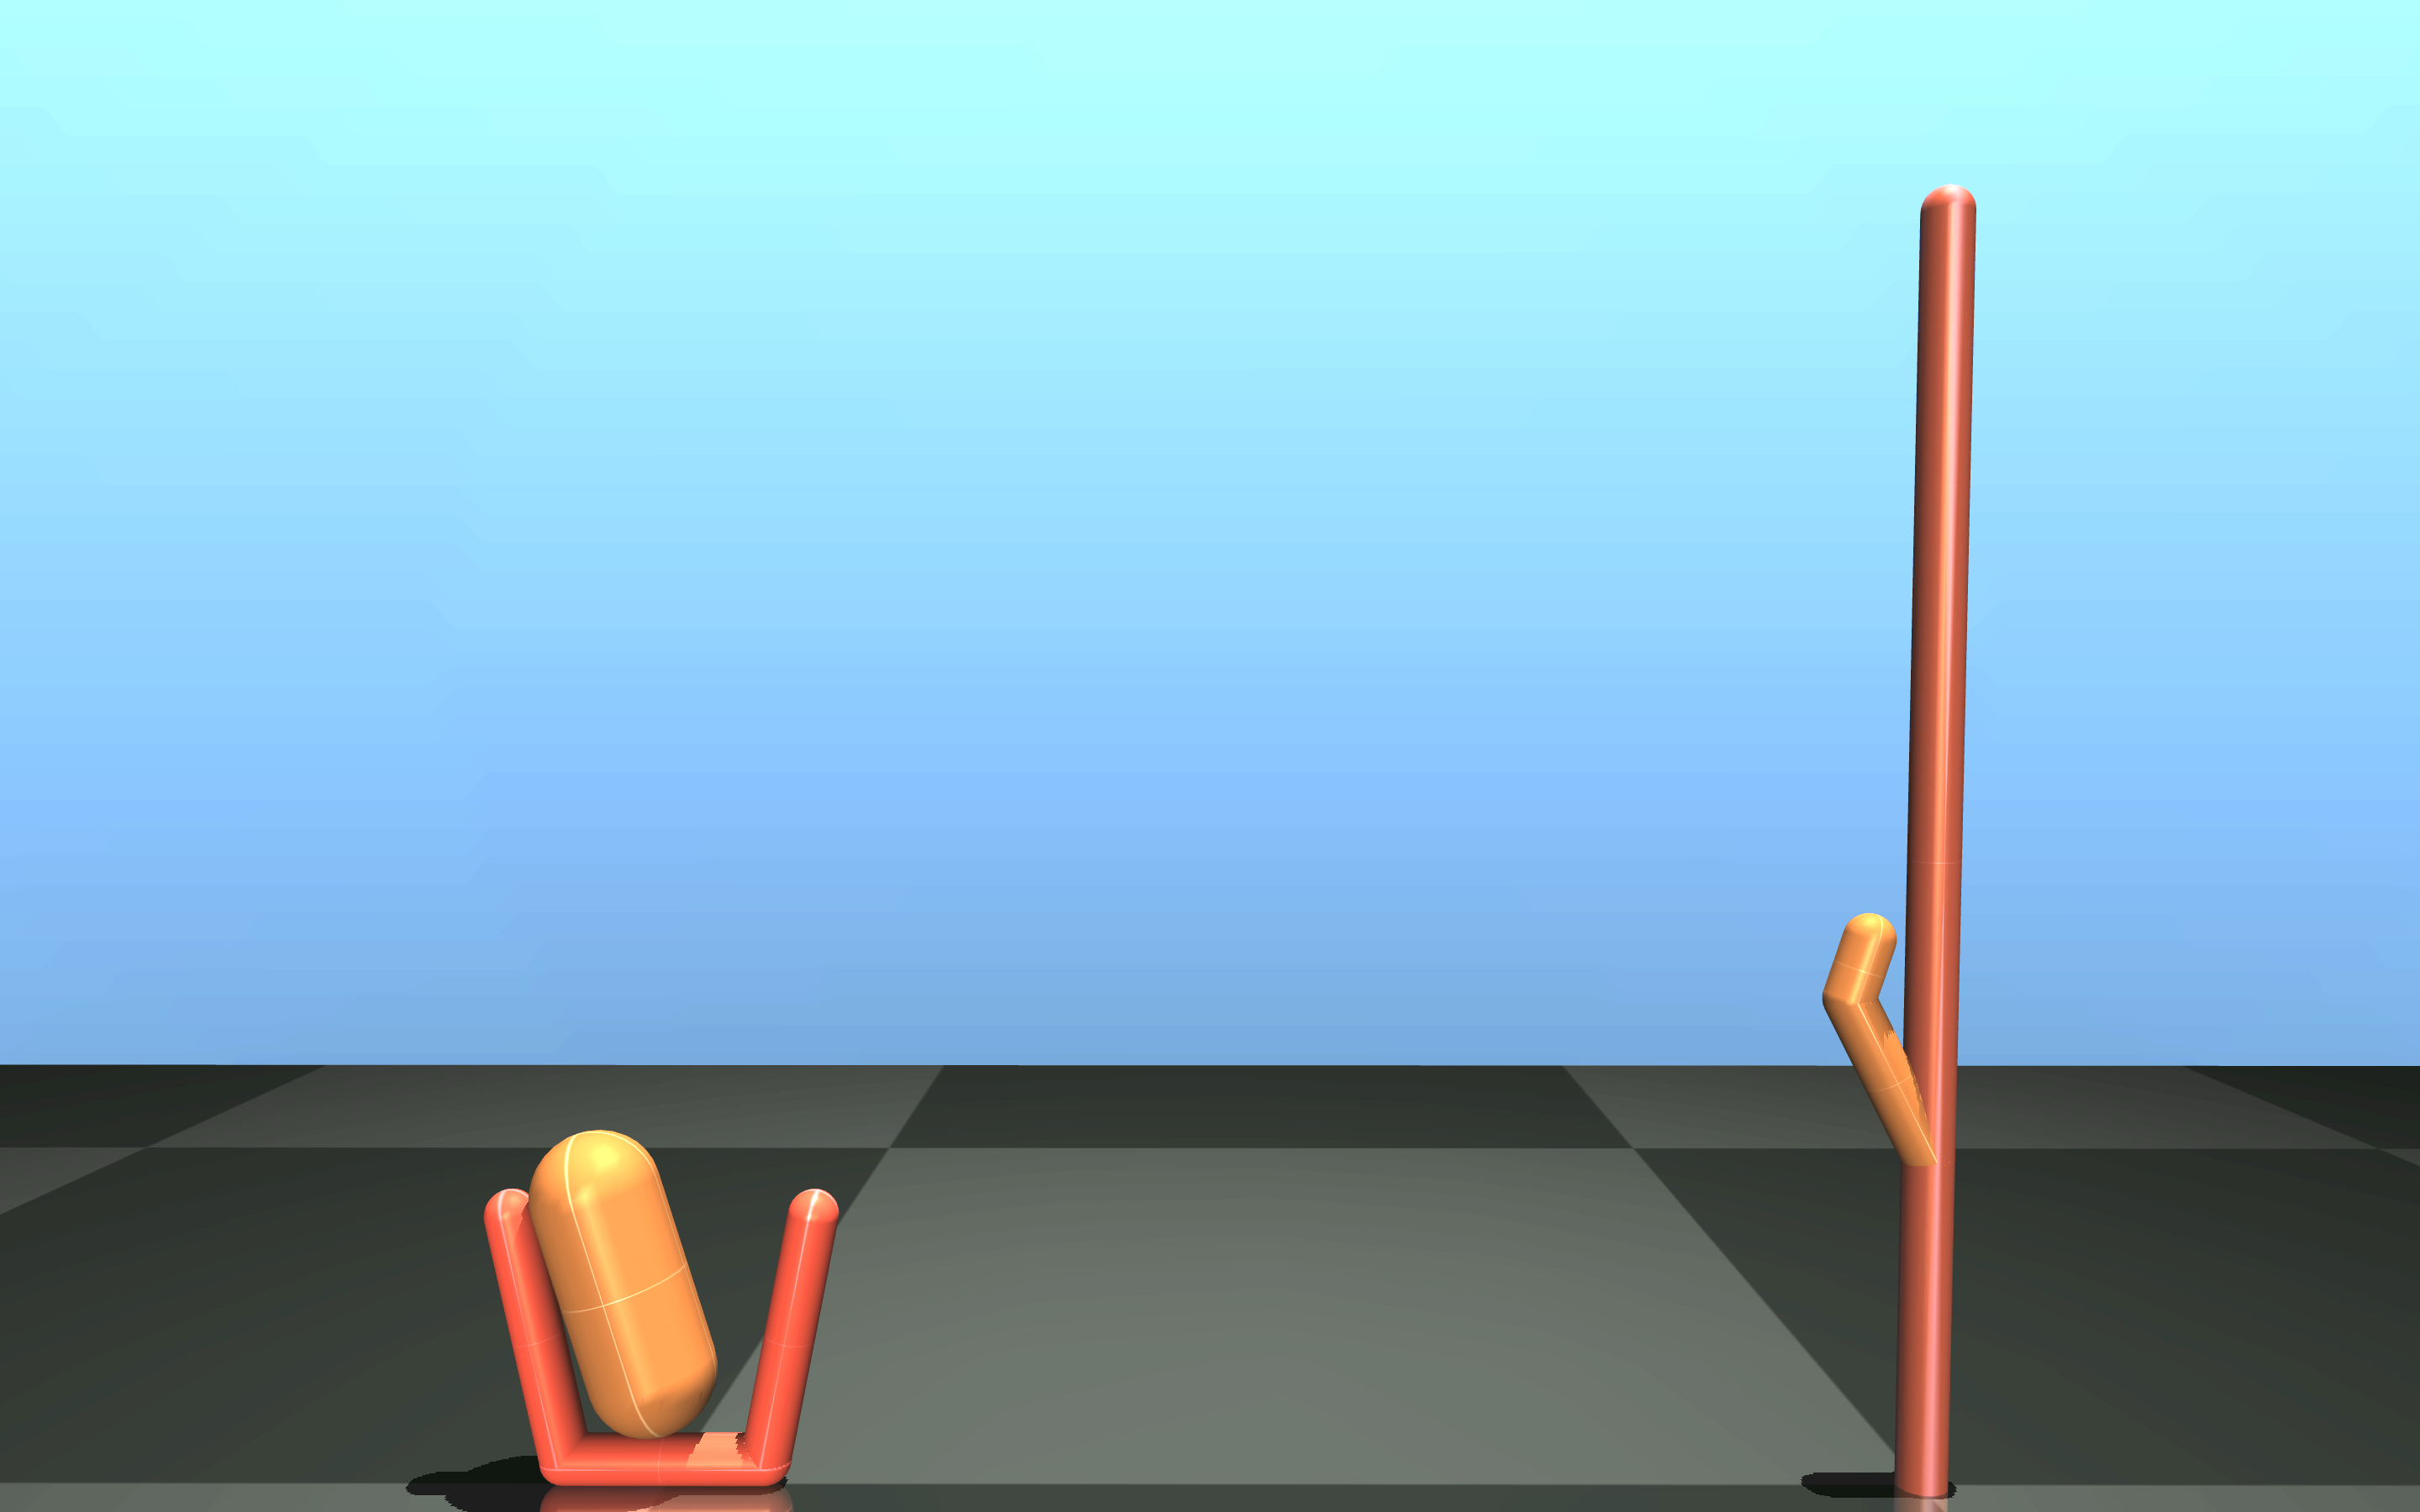
\includegraphics[width=0.24\textwidth]{figures/tosser/tosser4.png}
        \vspace{-0.5cm}
        \caption{ }
        \label{fig:tosser:im}
    \end{subfigure}
    
    % \vspace{-0.2cm}
    \begin{subfigure}[t]{0.24\textwidth}
        \centering
        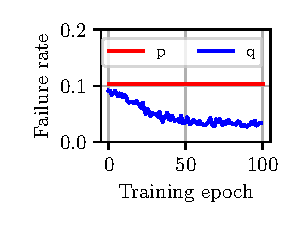
\includegraphics[width=\textwidth]{figures/tosser/TosserNF_cluster_2019_09_28_09_45_55/tosser_nf_bot_rate.pdf}
        \vspace{-0.8cm}
        \caption{ }
        \label{fig:tosser:ar}
    \end{subfigure}%
    ~ 
    \begin{subfigure}[t]{0.24\textwidth}
        \centering
        \includegraphics[width=\textwidth]{figures/tosser/TosserNF_cluster_2019_09_28_09_45_55/tosser_smc_variance_plot.pdf}
        \vspace{-0.8cm}
        \caption{ }
        \label{fig:tosser:smc:var}
    \end{subfigure}
    
    \begin{subfigure}[t]{0.48\textwidth}
        \centering
        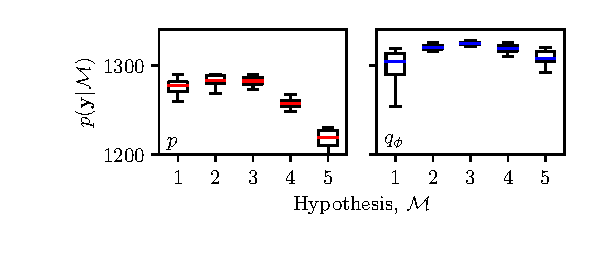
\includegraphics[width=\textwidth]{./figures/tosser/TosserNF_cluster_2019_09_28_09_45_55/tosser_box_plot.pdf}
        % \vspace{-1cm}
        \caption{ }
    \label{fig:tosser_hyp}
    \end{subfigure}
    \vspace{-0.2cm}
    \caption{Results of the ``tosser'' experiment introduced in Section \ref{sec:experiments:tosser}.
    \ref{fig:tosser:im} shows the evolution of state over time.
    \ref{fig:tosser:ar} shows the AF we learn markedly reduces the number of rejections.
    \ref{fig:tosser:smc:var} shows the results of performing SMC using the \emph{a priori} specified proposal and our learned autoregressive flow. 
    The autoregressive flow attains a much lower variance estimate, with a p-value of less than $0.0001$ in a paired t-test, indicating a strong statistical difference in performance.
    \ref{fig:tosser_hyp} shows the results of performing hypothesis testing, where hypothesis $3$ is correct, under a uniform prior over hypothesis. 
    The incorrect hypothesis is selected using $p$, while using $q_{\phi}$ the correct hypothesis is selected, with a statistically significant confidence.
    }
    \label{fig:tosser}
\end{figure}

Figure \ref{fig:tosser} shows the results of this experiment.
The capsule is mostly in free space resulting in an average rejection rate under $p$ of $10\%$.
Figure \ref{fig:tosser:ar} shows that the autoregressive flow learns a proposal with a lower rejection rate, reaching $3\%$ rejection.
However these rejections are concentrated in the critical regions of state-space, where chaotic behavior occurs, and so this reduction yields an large reduction in the variance of the evidence approximation, as shown in Figure \ref{fig:tosser:smc:var}.

\begin{figure}[t]
\centering
    \begin{subfigure}[t]{0.24\textwidth}
        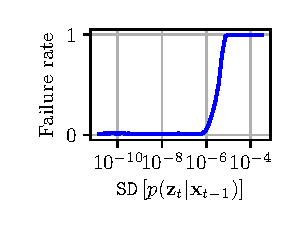
\includegraphics[width=\textwidth]{figures/bot_rate/bot_rate.pdf}
        \vspace{-0.8cm}
        \caption{}
        \label{fig:wormsim:bot_rate}
    \end{subfigure}%
    ~%
    \begin{subfigure}[t]{0.24\textwidth}
        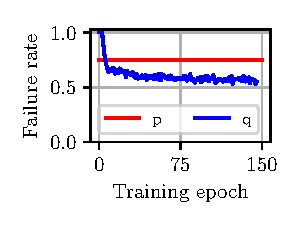
\includegraphics[width=\textwidth]{figures/bot_rate/wormsim_nf_bot_rate.pdf}
        \vspace{-0.8cm}
        \caption{}
        \label{fig:wormsim:bot_nf_rate}
    \end{subfigure}
\vspace{-0.5cm}
\caption{Results from the WormSim example introduced in Section \ref{sec:sub:wormsim}.
\ref{fig:wormsim:bot_rate} shows the rate at which the simulator fails increases sharply as a function of the standard deviation of the applied perturbation. 
\ref{fig:wormsim:bot_nf_rate} shows the reduction in rejections during training.
}
\label{fig:bot}
\end{figure}

We conclude this example by evaluating our method on hypothesis testing using pseudo-marginal evidence estimates.
The results for this are shown in Figure \ref{fig:tosser_hyp}.
We test $5$ different hypothesis of the mass of the capsule.
Using $p$ results in higher variance evidence approximations than when $q_{\phi}$ is used. 
Additionally, under $p$ the wrong model is selected ($2$ instead of $3$), although with low significance ($p=0.125$), while using $q_{\phi}$ selects the correct hypothesis with $p=0.0127$.
For this experiment we note that $q_{\phi}$ was trained on a single value of mass, and that this ``training mass'' was different to the ``testing mass.''
We believe this contributes to the increased variance in hypothesis $1$, which is very light compared to the training mass.
Training a $q_{\phi}$ with a further level of amortization over different mass values would further increase the fidelity of the model selection.
This is intimately linked with the larger project of jointly learning the model, and so we defer investigation to future works.

\subsection{Neuroscience Simulator}
\label{sec:sub:wormsim}
We conclude by applying our algorithm to a simulator for the widely studied \emph{Caenorhabditis elegans} roundworm.
WormSim, presented by \citet{boyle2012gait}, is a simulator of the locomotion of the worm, using a $510$ dimensional state representation.
We apply perturbations to a $98$ dimensional subspace defining the physical position of the worm, while conditioning on the full $510$ dimensional state vector.
The expected rate of failure increases sharply as a function of the scale of the perturbation applied, as shown in Figure \ref{fig:wormsim:bot_rate}, as the integrator used in WormSim is unable to integrate highly perturbed states.

The rejection rate during training is shown in Figure \ref{fig:wormsim:bot_nf_rate}.
We are able to learn an autoregressive flow with lower rejection rates, reaching approximately $53\%$ rejection, when $p$ has approximately $75\%$ rejection.
Although the rejection rate is higher than ultimately desired, we include this example as a demonstration of how rejections occur in simulators through integrator failure.
We believe larger flows with regularized parameters can reduce the rejection rate further.
